\documentclass[border=5pt]{standalone}
\usepackage{tikz}
\usepackage{amsmath}
\begin{document}
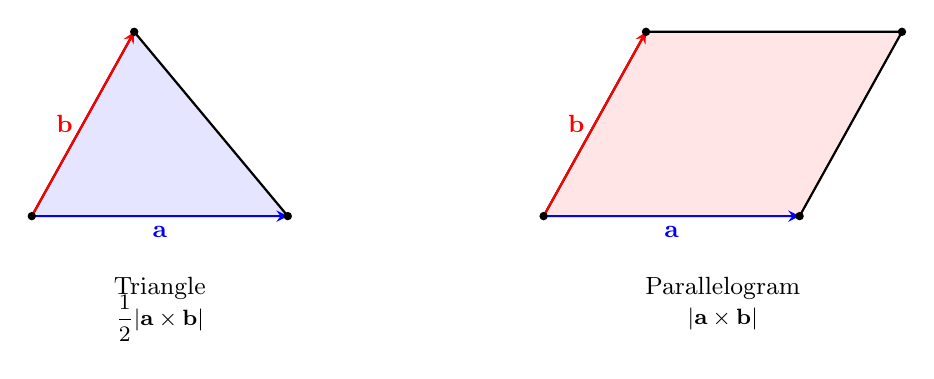
\begin{tikzpicture}[scale=1.3, >=stealth]
  % Two diagrams: triangle and parallelogram

  % Left: Triangle
  \begin{scope}[shift={(-3,0)}]
    \coordinate (A) at (0,0);
    \coordinate (B) at (2.5,0);
    \coordinate (C) at (1,1.8);
    \fill[blue!10] (A) -- (B) -- (C) -- cycle;
    \draw[thick] (A) -- (B) -- (C) -- cycle;
    \draw[->, thick, blue] (A) -- (B) node[midway, below, font=\small] {$\mathbf{a}$};
    \draw[->, thick, red] (A) -- (C) node[midway, left, font=\small] {$\mathbf{b}$};
    \filldraw[black] (A) circle (1pt);
    \filldraw[black] (B) circle (1pt);
    \filldraw[black] (C) circle (1pt);
    \node[below, font=\small] at (1.25, -0.5) {Triangle};
    \node[font=\footnotesize] at (1.25, -1.0) {$\dfrac{1}{2}|\mathbf{a}\times\mathbf{b}|$};
  \end{scope}

  % Right: Parallelogram
  \begin{scope}[shift={(2,0)}]
    \coordinate (A) at (0,0);
    \coordinate (B) at (2.5,0);
    \coordinate (C) at (3.5,1.8);
    \coordinate (D) at (1,1.8);
    \fill[red!10] (A) -- (B) -- (C) -- (D) -- cycle;
    \draw[thick] (A) -- (B) -- (C) -- (D) -- cycle;
    \draw[->, thick, blue] (A) -- (B) node[midway, below, font=\small] {$\mathbf{a}$};
    \draw[->, thick, red] (A) -- (D) node[midway, left, font=\small] {$\mathbf{b}$};
    \filldraw[black] (A) circle (1pt);
    \filldraw[black] (B) circle (1pt);
    \filldraw[black] (C) circle (1pt);
    \filldraw[black] (D) circle (1pt);
    \node[below, font=\small] at (1.75, -0.5) {Parallelogram};
    \node[font=\footnotesize] at (1.75, -1.0) {$|\mathbf{a}\times\mathbf{b}|$};
  \end{scope}
\end{tikzpicture}
\end{document}
